\documentclass[12pt]{article}
\usepackage{amsmath}
\usepackage{graphicx}
\usepackage{hyperref}
\usepackage[utf8]{inputenc}
\usepackage{geometry}
\usepackage{mathtools}
\usepackage{empheq}
\usepackage{listings}
\usepackage{xcolor}
\usepackage{authblk}
\usepackage{subcaption}
\usepackage{svg}
\usepackage{minted}


\definecolor{LightGray}{gray}{0.9}

\graphicspath{ {./assets/} }
\geometry{margin=0.75in}

\title{HW}
\date{}

\begin{document}

\begin{enumerate}

    \newpage
    \item Problem 1
    
    a.

    \begin{align*}
        E &= \frac{n^2 h^2}{8 m L^2} \\
        E &= \frac{1^2 \cdot \left(6.626 \cdot 10^{-34}\right)}{8 \cdot 9.109 \cdot 10^{-31} \cdot \left(10 \cdot 10^{-10}\right)} \\
        \Aboxed{E &= 6.02 \cdot 10^{-20} \text{ J}} \\
        E &= \frac{6.02 \cdot 10^{-20} \text{ J}}{1.602 \cdot 10^{-19} \text{ J/eV}} \\
        \Aboxed{E &= 0.376 \text{ eV}} \\
        E &= h\nu \\
        \tilde{\nu} &= \frac{\nu}{c} \\
        \tilde{\nu} &= \frac{E}{hc} \\
        \tilde{\nu} &= \frac{6.02 \cdot 10^{-20}}{6.626 \cdot 10^{-34} \cdot 3 \cdot 10^{-10}} \\
        \Aboxed{\tilde{\nu} &= 3031 \text{ cm$^-1$}}
    \end{align*}

    b. 

    \begin{align*}
        \psi &= \sqrt{\frac{2}{L}} \sin\left(\frac{n\pi x}{L}\right) \\
        \psi^*\psi dL &= \frac{2}{L} \sin^2\left(\frac{n\pi x}{L}\right) dL \\
        \intertext{n=2}
        \psi^*\psi dL &= \frac{2}{10\cdot10^{-10}} \sin^2\left(\frac{2\pi \cdot 5\cdot10^{-10}}{10\cdot10^{-10}}\right) dL \\
        \Aboxed{\psi^*\psi dL &= 0} \\
        \intertext{n=3}
        \psi^*\psi dL &= \frac{2}{10\cdot10^{-10}} \sin^2\left(\frac{3\pi \cdot 5\cdot10^{-10}}{10\cdot10^{-10}}\right) dL \\
        \Aboxed{\psi^*\psi dL &= 2\cdot10^9 dL}
    \end{align*}

    c. 

    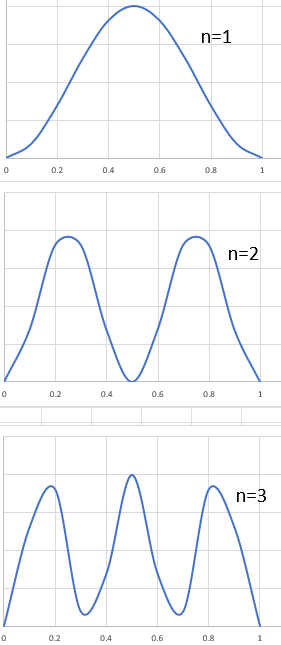
\includegraphics[width=0.5\textwidth]{assets/p1c.png}

    Plots above are $\psi^*\psi$ v Fraction of L. For n=2, the proability of an electron being at 0.5L is zero. So the probability of the transition from n=2 to n=3 would be 0.

    \newpage
    \item Problem 2 (4.3)
    
    a. 

    \begin{align*}
        \Delta E &= E_2 - E_1 \\
        E &= \frac{h^2n^2}{*ml^2} \\
        \Delta E &= \frac{h^2n_2^2}{8ml^2} - \frac{h^2n_1^2}{8ml^2} = \frac{h^2}{8ml^2} \left(n_2^2 - n_1^2\right) \\
        E &= h\nu \\
        c &= \lambda \nu \\
        \nu &= \frac{c}{\lambda} \\
        E &= \frac{hc}{\lambda} \\
        \frac{hc}{\lambda} &= \frac{h^2}{8ml^2} \left(n_2^2 - n_1^2\right) \\
        \Aboxed{\lambda &= \frac{8mL^2c}{h\left(n_2^2 - n_1^2\right)}}
    \end{align*}

    b.

    \begin{align*}
        \lambda &= \frac{8 \cdot 9.109 \cdot 10^{-31} \cdot \left(10\cdot10^{-10}\right) \cdot 3 \cdot 10^8}{6.626 \cdot 10^{-34} \cdot \left(2^2 - 1^2\right)} \\
        \lambda &= 1.10\cdot10^{-6} \text{ m} \\
        \Aboxed{\lambda &= 1099.84\text{ nm} }
    \end{align*}

    \newpage
    \item Problem 3
    
    a. Reduced mass for HBr

    \begin{align*}
        & m_{\text{H}} = 1.007875 \text{ amu} \\
        & m_{\text{Br}} = 80.916290 \text{ amu} \\ 
        \mu &= \frac{m_1m_2}{m_1 + m_2} \\
        \mu &= \frac{1.007875 \text{ amu} \cdot 80.916290 \text{ amu}}{1.007875 \text{ amu} + 80.916290 \text{ amu}} \\
        \Aboxed{\mu &= 0.995427 \text{ amu}}
    \end{align*}

    b. Find force constant k

    \begin{align*}
        & \text{Vibration frequency} = 2558.5 \text{ cm$^{-1}$} \\
        \omega &= \sqrt{\frac{k}{\mu}} \\
        k &= \omega \mu \\
        \nu &= \frac{c}{\lambda} \\
        \nu &= c \tilde{\nu} \\
        \nu &= 3\cdot10^{10} \text{ cm/s} \cdot 2558.5 \text{ cm$^{-1}$} \\
        \Aboxed{\nu &= 7.6755\cdot10^{13}} \\
        \omega &= 2\pi\nu \\
        \omega &= 2\pi \cdot 7.6755\cdot10^{13} \\
        \Aboxed{\omega &= 4.823\cdot10^{14}} \\
        k &= \omega \mu \\
        k &= \left(4.823\cdot10^{14}\right)^2 \cdot \frac{0.995427}{6.022\cdot10^{26}} \\
        \Aboxed{k &= 384.5 \text{ kg/s$^2$}}
    \end{align*}

    c. Given R = 141.4 pm, find moment of inertia

    \begin{align*}
        I &= \mu R^2 \\
        I &= \frac{0.995427}{6.022\cdot10^{26}} \left(141.4\cdot10^{12}\right) \\
        \Aboxed{I &= 3.305\cdot10^{-47} \text{ kg$\cdot$m$^2$}}
    \end{align*}

    d.

    \begin{align*}
        \hbar &= \frac{h}{2\pi} = 1.0547\cdot10^{-34} \text{ J$\cdot$s} \\
        B &= \frac{\hbar^2}{2I} \\
        B &= \frac{\left(1.0547\cdot10^{-34} \text{ J$\cdot$s}\right)^2}{2 \cdot 3.305\cdot10^{-47} \text{ kg$\cdot$m$^2$}} \\
        \Aboxed{B &= 1.683\cdot10^{-22} \text{ J}} \\
        \nu &= \frac{E}{h} \\
        \nu &= \frac{1.683\cdot10^{-22} \text{ J}}{6.626\cdot10^{-34} \text{ J$\cdot$s}} \\
        \Aboxed{\nu &= 2.54\cdot10^{11} \text{ s$^{-1}$}} \\
        \intertext{0 to 1 is at 2B}
        \nu &= 2 \cdot 2.54\cdot10^{11} \text{ s$^{-1}$} \\
        \Aboxed{\nu &= 5.08\cdot10^{11} \text{ s$^{-1}$}} \\
        \intertext{1 to 2 is at 4B}
        \nu &= 4 \cdot 2.54\cdot10^{11} \text{ s$^{-1}$} \\
        \Aboxed{\nu &= 1.016\cdot10^{12} \text{ s$^{-1}$}}
    \end{align*}

    \newpage
    \item Problem 4 (4.9)
    
    a.
    
    \begin{align*}
        \omega &= \sqrt{\frac{k}{\mu_m}} = 2\pi\nu \\
        \nu &= \frac{1}{2\pi}\sqrt{\frac{k}{\mu_m}} \\
        \nu &= \frac{1}{2\pi}\sqrt{\frac{1903.17}{1.1385\cdot10^{-36}}} \\
        \Aboxed{\nu &= 6.5072\cdot10^{13} \text{ s$^{-1}$}} \\
        \tilde{\nu}_{\text{HO}} &= \frac{6.5072\cdot10^{13} \text{ s$^{-1}$}}{3\cdot10^{10} \text{ cm/s}} \\
        \Aboxed{\tilde{\nu}_{\text{HO}} &= 2170.56 \text{ cm$^{-1}$}}
    \end{align*}

    b. The value we get for $\tilde{\nu_{\text{HO}}} = 2170.56 \text{ cm$^{-1}$}$ while the spectroscopically measured one is $\tilde{\nu_{\text{HO}}} = 2143.36 \text{ cm$^{-1}$}$. Our value is larger than the measured, and the reason for this difference is due to the anharmonicity of CO. The spaces between n=0 and 1 are closer than expected for harmonic oscillators.
    
    \newpage
    \item Problem 5 (4.12)
    
    a. 

    \begin{align*}
        \Delta E &= h\nu \\
        \omega &= \sqrt{\frac{k}{m}} = 2\pi\nu \\
        \nu &= \frac{1}{2\pi}\sqrt{\frac{k}{m}} \\
        \nu &= \frac{\Delta E}{h} \\
        \nu &= \frac{4.25 \cdot 10^{-21}}{6.626\cdot10^{-34}} \\
        \nu &= 6.41 \cdot 10^{12} \text{ s$^{-1}$} \\
        \sqrt{\frac{k}{m}} &= 2\pi \cdot 6.41 \cdot 10^{12} \text{ s$^{-1}$} \\
        \sqrt{\frac{k}{m}} &= 4.03 \cdot 10^{12} \text{ rad/s} \\
        k &= \left(4.03 \cdot 10^{12}\right) 3.15 \cdot 10^{-25} \\
        \Aboxed{k &= 512 \text{ N/m} }
    \end{align*}

    b.

    \begin{align*}
        2\pi\nu &= \sqrt{\frac{k}{m}} \\
        k &= \left(2\pi\nu\right)^2 m \\
        k &= \left(2\pi\cdot 0.805\right)^2 \cdot 20 \\
        \Aboxed{k &= 512 \text{ N/m} }
    \end{align*}

    c. The reason it is said that the chemical bond is compared to a mechanical spring, this is in characteristic that the chemical bond acts like a very strong spring. In essence, the spring in (b) holds 20 kg mass.
    
    \newpage
    \item Problem 6 (4.19)
    
    \begin{align*}
        \mu_{\text{H}_2} &= \frac{1\cdot1}{1+1} = \frac{1}{2} \\
        \mu_{\text{HD}} &= \frac{1\cdot2}{1+2} = \frac{2}{3} \\
        \mu_{\text{O}_2} &= \frac{2\cdot2}{2+2} = 1 \\
        \mu_{\text{HD}} &= \frac{4}{3} \mu_{\text{H}_2} \\
        \mu_{\text{D}_2} &= 2 \mu_{\text{H}_2} \\
        \omega &= \sqrt{\frac{k}{\mu_m}} 2\pi\nu = 2\pi c\tilde{\nu} \\
        \tilde{\nu}_{\text{H}} &= \sqrt{\frac{3}{4}} \tilde{\nu}_{\text{H}_2} \\
        \tilde{\nu}_{\text{HD}} &= \sqrt{\frac{3}{4}} \cdot 4400 \\
        \Aboxed{\tilde{\nu}_{\text{HD}} &= 3811 \text{ cm$^{-1}$}} \\
        \tilde{\nu}_{\text{D}_2} &= \sqrt{\frac{1}{2}} \tilde{\nu}_{\text{H}_2} \\
        \tilde{\nu}_{\text{D}_2} &= \sqrt{\frac{1}{2}} \cdot 4400 \\
        \Aboxed{\tilde{\nu}_{\text{D}_2} &= 3111 \text{ cm$^{-1}$}}
    \end{align*}

\end{enumerate}

\end{document}